%\documentclass[tikz, border=5pt]{standalone}
\begin{document}
	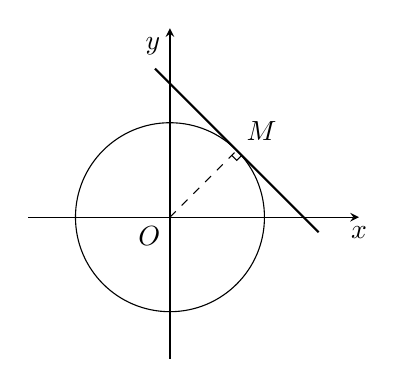
\begin{tikzpicture}[>=stealth, scale=0.6]
		% 绘制坐标轴
		\draw[->] (-3,0) -- (4,0) node[below ] {$x$};
		\draw[->] (0,-3) -- (0,4) node[below left] {$y$};
		\node at (0,0) [below left] {$O$};
		
		% 绘制圆(圆心在原点,半径设为2)
		\draw (0,0) circle (2);
		
		% 定义切点M的坐标(M(√2, √2),在圆上且位于第一象限)
		\coordinate (M) at ({sqrt(2)},{sqrt(2)});
		
		% 绘制从原点到切点M的线段(虚线)
		\draw[dashed] (0,0) -- (M);
		
		% 绘制切线(过M且与OM垂直,斜率为-1)
		\draw[thick] (M) -- ++({-sqrt(3)},{sqrt(3)}) (M) -- ++({sqrt(3)},{-sqrt(3)});
		
		% 标记切点M
		\node at (M) [above right] {$M$};
		
		% 绘制直角符号
		\draw ({sqrt(2)},{sqrt(2)}) -- ++ (-45: 0.15) -- ++ (-135: 0.15) -- ++ (135: 0.15) ;
		
	\end{tikzpicture}
\end{document}
